\section{Komputer Kuantum}
Dalam pencarian keadaan dasar Hamiltonian Ising, diperlukan komputasi yang mampu memecahkan masalah optimasi kombinatorial yang kompleks. Komputasi klasik dapat membantu memecahkan masalah kombinatorial namun memiliki keterbatasan dalam memecahkan masalah saat menghadapi kompleksitas permasalahan yang terlalu tinggi. Komputer kuantum diimplementasikan untuk mengatasi hal tersebut lewat pengukuran energi kombinasi yang ada dari pemodelan Hamiltonian \textit{Ising} yang sudah terkonstruksi. Selain itu, komputer kuantum dapat memproses dan memanipulasi informasi dalam ruang Hilbert yang sangat luas menggunakan rangkaian kuantum khusus lewat gerbang kuantum yang sangat berbeda dari gerbang klasik. Komputer kuantum memanfaatkan prinsip superposisi dan keterbelitan kuantum untuk menavigasi ruang solusi dari masalah optimasi kombinatorial kompleks yang mana sangat sulit dijangkau oleh sistem komputasi klasik \cite{preskill_quantum_2018}.

Aplikasi teknologi kuantum dapat membuka peluang rekonstruksi portofolio keuangan dengan pendekatan ekonofisika yang mengasumsikan interaksi dinamis aset setara dengan konfigurasi spin partikel dalam ruang fisis. Kendala dimensi ruang pencarian yang melekat pada algoritma optimasi konvensional dapat diatasi melalui sifat fundamental komputasi kuantum yaitu superposisi dan keterbelitan kuantum yang mana pemrosesan informasi dilakukan secara paralel. Bab ini akan menguraikan secara mendalam bagaimana sistem qubit dapat menjadi fondasi utama teknis komputer kuantum lalu dilanjutkan dengan gerbang kuantum 1 qubit dan 2 qubit. Kemudian dikenalkan pula Quantum entanglement sebagai akibat dari penggunaan gerbang kuantum dan Quantum Measurement sebagai dasar pengukuran sistem kuantum di akhir rangkaian kuantum. Terakhir, Quantum Machine Learning dan Quantum Deep Learning yang menjadi dasar dari algoritma VQE yang akan digunakan pada tugas akhir ini.

\subsection{Sistem Qubit}
\textit{Qubit} didefinisikan sebagai satuan informasi dasar dalam komputasi kuantum yang memperluas konsep bit klasik menjadi sistem dua-keadaan mekanika kuantum sehingga mampu eksis dalam kondisi superposisi. Berbeda dengan bit klasik yang hanya memiliki dua status 0 dan 1 secara eksklusif, \textit{qubit} didefinisikan secara matematis melalui vektor kolom di ruang vektor kompleks dua-dimensi $\mathbb{C}^2$ \cite{nielsen_quantum_2010}. Qubit dapat direpresentasikan dengan basis komputasi ortogonal $|0\rangle$ dan $|1\rangle$ yang dinyatakan melalui vektor kolom ortonormal dengan bentuk matematis
\begin{equation}
\label{eq:basis_keadaan}
|0\rangle = \begin{pmatrix} 1 \\ 0 \end{pmatrix}, \quad |1\rangle = \begin{pmatrix} 0 \\ 1 \end{pmatrix}.
\end{equation}
Keberadaan vektor keadaan \textit{qubit} yang bersifat superposisi dinyatakan pada persamaan gelombang ($\psi$) dari keadaan qubit dengan bentuk 
\begin{equation}
    |\psi\rangle = \alpha |0\rangle + \beta |1\rangle
\end{equation}
di mana $\alpha$ dan $\beta$ merupakan amplitudo probabilitas sistem kuantum berada di keadaan $|0\rangle$ dan $|1\rangle$. Karena sistem fisik harus memenuhi syarat kekekalan probabilitas yang menyatakan bahwa total probabilitas dari keadaan $|0\rangle$ dan $|1\rangle$ harus bernilai 1 yang berarti pasti ada, dengan bentuk persamaan 
\begin{equation}
    |\alpha|^2 + |\beta|^2 = 1
\end{equation}
dimana kuadrat dari amplitudo probabilitas menyatakan peluang sistem kuantum berada di keadaan $|0\rangle$ dan $|1\rangle$ yang bernilai 0 hingga 1. Sifat superposisi inilah yang memungkinkan \textit{qubit} berada dalam kombinasi linier dari kedua basis keadaan dalam satu waktu yang sama, sehingga memberikan potensi komputasi paralel yang jauh melampaui kapabilitas bit klasik.

Keadaan sebuah \textit{qubit} dapat direpresentasikan menggunakan representasi Bola \textit{Bloch} yang memvisualisasikan bagaimana vektor keadaan sebuah qubit terletak di dalam ruang keadaan 3D.
\begin{figure}[htbp]
    \centering
    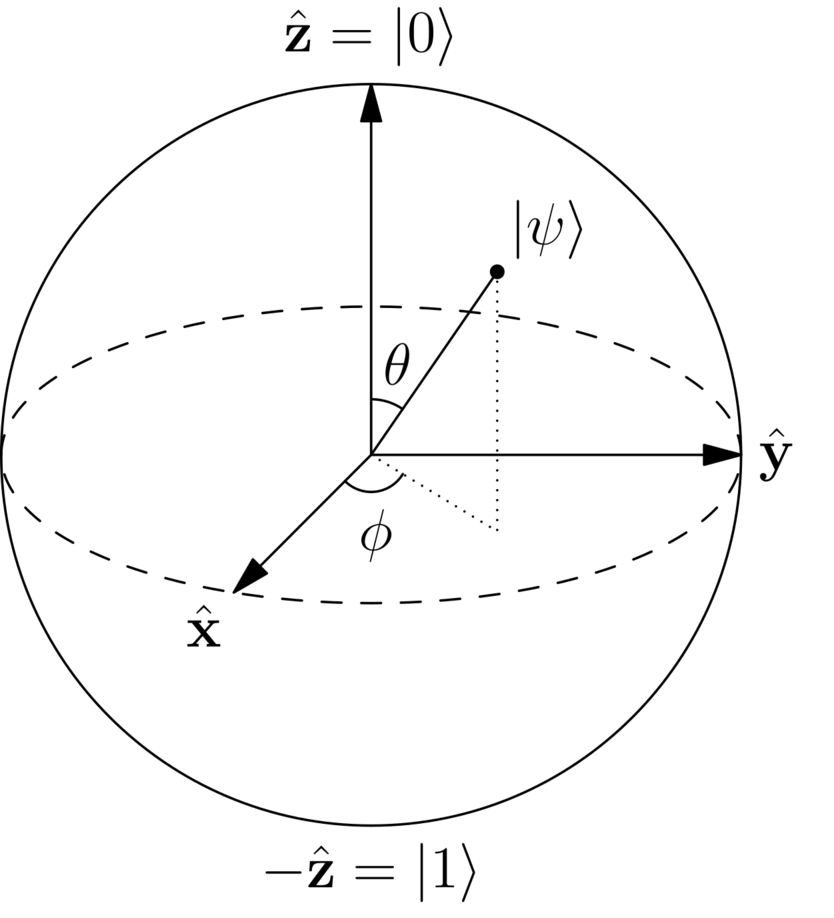
\includegraphics[width=0.45\textwidth]{Images/bloch_sphere.png}
    \caption{Visualisasi Bola Bloch sebagai representasi geometris dari status \textit{qubit} dalam ruang parameter kontinu.}
    \label{fig:bloch_sphere}
\end{figure}
Pada gambar \ref{fig:bloch_sphere}, vektor keadaan pada sebuah qubit direpresentasikan oleh arah garis $|\psi\rangle$ dari tengah menuju permukaan bola. Vektor tersebut dipengaruhi oleh dua komponen yaitu parameter polar $\theta$ yang bergantung pada amplitudo probabilitas dan parameter azimutal sebagai fase relatif $\phi$. Ketika vektor keadaan bergerak dari kutub utara menuju kutub selatan sepanjang sumbu z, probabilitas pengukuran pada basis komputasi berubah secara kontinu dari keadaan $|0\rangle$ menjadi $|1\rangle$. Sementara itu, semua keadaan yang terletak pada ekuator Bola Bloch memiliki probabilitas pengukuran yang sama, yaitu 0,5 untuk $|0\rangle$ dan 0,5 untuk $|1\rangle$, namun dibedakan oleh fase relatif yang dinyatakan oleh sudut $\phi$.

Secara aljabar, posisi geometris dari vektor keadaan tersebut dapat dipetakan ke dalam koordinat Kartesian tiga dimensi pada ruang bola Bloch. Koordinat Kartesian $x$, $y$, dan $z$ dari titik ujung vektor keadaan didefinisikan secara unik melalui hubungan sudut polar $\theta$ dan sudut azimutal $\phi$ sebagai berikut:
\begin{equation}
\label{eq:koordinat_kartesian_bloch}
x = \sin\theta\cos\phi, \quad y = \sin\theta\sin\phi, \quad z = \cos\theta.
\end{equation}
Hubungan koordinat spasial tersebut memetakan ruang status Hilbert dua dimensi ke dalam representasi ruang nyata tiga dimensi secara konsisten untuk mempermudah visualisasi fisis. Melalui pemetaan tersebut, visualisasi lintasan evolusi keadaan qubit di bawah pengaruh gerbang kuantum dapat dianalisis dengan lebih intuitif dan sistematis.

\subsection{Manipulasi Informasi pada Gerbang 1 Qubit}
Manipulasi informasi dalam arsitektur komputasi kuantum dilakukan secara esensial melalui penerapan berbagai gerbang logika yang direpresentasikan sebagai operator uniter U pada ruang vektor kompleks dua dimensi. Secara matematis, representasi matriks uniter paling umum untuk gerbang satu qubit diformulasikan melalui parameterisasi fisis yang melibatkan sudut rotasi θ dan tiga parameter fase kompleks independen yaitu $\alpha$, $\beta$, serta $\gamma$. Konfigurasi operasional dari parameterisasi matriks uniter tersebut dinyatakan ke dalam sebuah representasi persamaan matematis yang merepresentasikan transformasi kuantum umum
\begin{equation}
\label{eq:unitary_general}
U = e^{i\alpha} \begin{pmatrix} e^{i\beta}\cos\theta & e^{i\gamma}\sin\theta \\ -e^{-i\gamma}\sin\theta & e^{-i\beta}\cos\theta \end{pmatrix}.
\end{equation}
Penjabaran mengenai proses parameterisasi matriks uniter dua dimensi tersebut dari definisi awal hingga bentuk ekuivalen akhir disajikan secara komprehensif pada Lampiran \ref{app:penurunan_gerbang_uniter}. Melalui pemanfaatan bentuk matriks umum tersebut, observasi fisis terhadap berbagai macam gerbang uniter dasar kuantum dapat didemonstrasikan secara sistematis hanya dengan menyesuaikan konfigurasi parameter fase $\alpha$, $\beta$, $\gamma$, dan
sudut rotasi fisis $\theta$.

Matriks Pauli-X yang bertindak sebagai operator pembalik status keadaan $|0\rangle$ ke $|1\rangle$ dan sebaliknya, dapat diperoleh dengan menetapkan nilai sudut rotasi $\theta$ sebesar $\pi/2$. Pemilihan parameter sudut tersebut berimplikasi pada hilangnya kontribusi fungsi trigonometri kosinus dan menyisakan fungsi sinus bernilai satu pada elemen matriks. Untuk menyesuaikan elemen matriks agar bernilai satu, parameter fase relatif $\gamma$ dipilih sebesar $\pi/2$ sedangkan fase $\beta$ diatur bernilai nol. Dengan menetapkan nilai fase global $\alpha$ sebesar minus $\pi/2$, diperoleh matriks Pauli-X:
\begin{equation}
X = e^{-i\pi/2} \begin{pmatrix} 0 & e^{i\pi/2} \\ -e^{-i\pi/2} & 0 \end{pmatrix} = -i \begin{pmatrix} 0 & i \\ i & 0 \end{pmatrix} = \begin{pmatrix} 0 & 1 \\ 1 & 0 \end{pmatrix}.
\end{equation}
Matriks Pauli-Y juga dapat diperoleh dengan penyesuaian parameter sudut dan fase dari representasi uniter umum. Nilai sudut polar $\theta$ kembali dipilih sebesar $\pi/2$, sedangkan parameter fase relatif $\gamma$ diatur bernilai nol dan fase $\beta$ diatur bernilai nol. Penetapan nilai parameter tersebut menghasilkan bentuk matriks uniter yang didominasi oleh elemen bernilai riil pada bagian diagonal kedua matriks tersebut. Selanjutnya, dengan mengimplementasikan nilai fase global $\alpha$ sebesar $\pi/2$, diperoleh matriks Pauli-Y dengan penyimpangan fase global sebesar minus satu:
\begin{equation}
e^{i\pi/2} \begin{pmatrix} 0 & 1 \\ -1 & 0 \end{pmatrix} = i \begin{pmatrix} 0 & 1 \\ -1 & 0 \end{pmatrix} = \begin{pmatrix} 0 & i \\ -i & 0 \end{pmatrix} = -Y.
\end{equation}
Sementara itu, matriks Pauli-Z yang merepresentasikan pergeseran fase relatif pada keadaan qubit dapat diturunkan dengan menetapkan parameter sudut rotasi $\theta$ bernilai nol. Pemilihan nilai parameter sudut tersebut mengakibatkan elemen di luar diagonal utama bernilai nol karena kontribusi fungsi trigonometri sinus yang menghilang. Untuk memunculkan perbedaan tanda pada diagonal utama matriks, parameter fase relatif $\beta$ dipilih sebesar $\pi/2$ sedangkan fase $\gamma$ bernilai bebas. Selanjutnya, dengan mengalikan matriks tersebut dengan fase global $\alpha$ sebesar minus $\pi/2$, diperoleh representasi matriks Pauli-Z secara presisi tanpa adanya faktor fase imajiner tambahan:
\begin{equation}
Z = e^{-i\pi/2} \begin{pmatrix} e^{i\pi/2} & 0 \\ 0 & e^{-i\pi/2} \end{pmatrix} = -i \begin{pmatrix} i & 0 \\ 0 & -i \end{pmatrix} = \begin{pmatrix} 1 & 0 \\ 0 & -1 \end{pmatrix}.
\end{equation}
Langkah penyesuaian parameter fase ini secara konsisten membuktikan bahwa seluruh operator Pauli dasar merupakan representasi uniter dari grup khusus kuantum.

Matriks Pauli dapat dihimpun dan dinotasikan dengan $\sigma_x$, $\sigma_y$, dan $\sigma_z$ yang tetap merupakan operator Hermitian dan uniter dengan bentuk 
\begin{equation}
\label{eq:matriks_pauli}
\sigma_x = \begin{pmatrix} 0 & 1 \\ 1 & 0 \end{pmatrix}, \quad \sigma_y = \begin{pmatrix} 0 & -i \\ i & 0 \end{pmatrix}, \quad \text{dan} \quad \sigma_z = \begin{pmatrix} 1 & 0 \\ 0 & -1 \end{pmatrix}.
\end{equation}
Setiap representasi matriks Pauli tersebut difungsikan secara komputasional untuk memanipulasi informasi pada suatu \textit{qubit} tunggal melalui mekanisme pemetaan basis keadaan secara deterministik~\cite{fedorov_vqe_2022,hidalgo_quantum_2006}. Secara fungsional, gerbang Pauli-X setara dengan gerbang NOT pada sistem komputasi klasik, di mana status keadaan dari $|0\rangle$ ditukar menjadi $|1\rangle$ dan sebaliknya melalui operasi uniter tersebut. Secara aljabar, aksi pemetaan fisis dari operator Pauli-X terhadap himpunan basis komputasi tersebut dapat dinyatakan secara komprehensif melalui relasi kesamaan fisis berikut:
\begin{equation}
\label{eq:aksi_paulix}
X|0\rangle = |1\rangle, \quad X|1\rangle = |0\rangle.
\end{equation}
Di sisi lain, gerbang Pauli-Y melakukan pertukaran status keadaan komputasi sekaligus memberikan fase kompleks imajiner pada konfigurasi amplitudo probabilitas \textit{qubit}. Karakteristik operasional dari gerbang Pauli-Y tersebut secara geometris merepresentasikan rotasi fisis sebesar $180^\circ$ terhadap sumbu-y pada koordinat bola Bloch, yang aksi pemetaannya secara matematis dirumuskan sebagai:
\begin{equation}
\label{eq:aksi_pauliy}
Y|0\rangle = i|1\rangle, \quad Y|1\rangle = -i|0\rangle.
\end{equation}
Sementara itu, stabilitas nilai amplitudo probabilitas pada setiap basis komputasi dipertahankan secara teknis oleh gerbang Pauli-Z, tetapi tanda fase relatif antara keadaan $|0\rangle$ dan $|1\rangle$ dibalikkan oleh operator tersebut. Mekanisme pergeseran fase asimetris tersebut direpresentasikan dengan rotasi sebesar $180^\circ$ terhadap sumbu-z pada ruang Hilbert melalui pemetaan fisis:
\begin{equation}
\label{eq:aksi_pauliz}
Z|0\rangle = |0\rangle, \quad Z|1\rangle = -|1\rangle.
\end{equation}

Selain variasi gerbang Pauli, gerbang Hadamard ($H$) direpresentasikan sebagai gerbang logika satu \textit{qubit} yang  mana berasal dari pencarian vektor eigen dari gerbang Pauli-X. Pencarian vektor eigen tersebut diawali dengan persamaan untuk mencari nilai eigen $\lambda$ dari matriks Pauli-X yang beroperasi di dalam ruang Hilbert dua dimensi. Nilai eigen dari sebuah operator kuantum dapat diperoleh dengan menghitung nilai determinan dari selisih antara matriks Pauli-X dan perkalian skalar matriks identitas yang disamakan dengan nilai nol~\cite{kumar_family_2025,sim_expressibility_2019}. Pencarian himpunan nilai eigen tersebut dapat dirumuskan melalui persamaan
\begin{equation}
\label{eq:eigen_value_x}
\det(X - \lambda I) = \det \begin{pmatrix} -\lambda & 1 \\ 1 & -\lambda \end{pmatrix} = \lambda^2 - 1 = 0.
\end{equation}
Sehingga diperoleh dua buah nilai eigen, yaitu $\lambda_1 = 1$ dan $\lambda_2 = -1$.

Setelah seluruh nilai eigen berhasil diperoleh, masing-masing vektor eigen dievaluasi dengan mensubstitusikan nilai $\lambda$ kembali ke dalam persamaan nilai eigen. Hubungan amplitudo antara komponen basis keadaan atas dan komponen basis keadaan bawah dihasilkan dari persamaan untuk representasi nilai eigen pertama bernilai $\lambda_1 = 1$~\cite{cohen_portfolio_2020}. Vektor eigen pertama yang mewakili keadaan kuantum positif dapat diperoleh dari persamaan
\begin{equation}
\label{eq:eigen_vector_1}
|+\rangle = \frac{1}{\sqrt{2}} \begin{pmatrix} 1 \\ 1 \end{pmatrix} = \frac{|0\rangle + |1\rangle}{\sqrt{2}}.
\end{equation}
Di sisi lain, sistem persamaan linier mengharuskan amplitudo dari komponen basis yang memiliki tanda sebaliknya memiliki nilai eigen kedua bernilai $\lambda_2 = -1$. Dengan syarat normalisasi, vektor eigen kedua yang merepresentasikan keadaan kuantum negatif dapat diperoleh lewat persamaan
\begin{equation}
\label{eq:eigen_vector_2}
|-\rangle = \frac{1}{\sqrt{2}} \begin{pmatrix} 1 \\ -1 \end{pmatrix} = \frac{|0\rangle - |1\rangle}{\sqrt{2}}.
\end{equation}
Hasil kedua vektor eigen yang saling ortogonal ini digunakan sebagai landasan utama untuk mendefinisikan susunan elemen matriks transformasi basis pada arsitektur sistem komputasi kuantum.

Representasi matriks dari gerbang uniter Hadamard dapat dikonstruksi dengan menyusun kedua vektor eigen hasil dari operator Pauli-X tersebut sebagai komponen kolom~\cite{wang_achieving_2025,li_ising_2023,datta_relationship_2015}. Sebuah bentuk perkalian konstanta terhadap elemen matriks yang memiliki konfigurasi tanda asimetris dapat diperoleh lewat mekanisme penyusunan vektor eigen ortogonal ini dengan relasi matematis
\begin{equation}
\label{eq:matriks_hadamard}
H = \begin{pmatrix} |+\rangle & |-\rangle \end{pmatrix} = \frac{1}{\sqrt{2}} \begin{pmatrix} 1 & 1 \\ 1 & -1 \end{pmatrix}.
\end{equation}
Dari konstruksi matriks tersebut, basis komputasi gerbang Hadamard menunjukkan suatu kombinasi linier dari superposisi untuk memfasilitasi algoritma komputasi yang bersifat paralel. Oleh karena itu, operator Hadamard dapat dipetakan terhadap masing-masing basis ortogonal di dalam ruang Hilbert dua dimensi melalui hubungan
\begin{equation}
\label{eq:aksi_hadamard}
H|0\rangle = \frac{|0\rangle + |1\rangle}{\sqrt{2}}, \quad H|1\rangle = \frac{|0\rangle - |1\rangle}{\sqrt{2}}.
\end{equation}
Representasi skematis dari operasi matriks Pauli dan gerbang Hadamard tersebut dapat divisualisasikan pada Gambar \ref{fig:gerbang_pauli}, di mana kotak berlabel $X$, $Y$, $Z$, dan $H$ menunjukkan masing-masing gerbang logika kuantum dasar yang bekerja pada alur data qubit.
\begin{figure}[htbp]
    \centering
    \begin{tikzpicture}[scale=1.3, >=stealth]
        % Gerbang X
        \draw (0,1) -- (2,1);
        \draw[fill=white] (0.6,0.7) rectangle (1.4,1.3) node[midway] {$X$};
        
        % Gerbang Y
        \draw (3,1) -- (5,1);
        \draw[fill=white] (3.6,0.7) rectangle (4.4,1.3) node[midway] {$Y$};
        
        % Gerbang Z
        \draw (6,1) -- (8,1);
        \draw[fill=white] (6.6,0.7) rectangle (7.4,1.3) node[midway] {$Z$};
        
        % Gerbang H
        \draw (9,1) -- (11,1);
        \draw[fill=white] (9.6,0.7) rectangle (10.4,1.3) node[midway] {$H$};
    \end{tikzpicture}
    \caption{Simbolisme gerbang Pauli dan gerbang Hadamard pada sirkuit kuantum yang merepresentasikan transformasi uniter dasar $X$, $Y$, $Z$, dan $H$ pada satu \textit{qubit}.}
    \label{fig:gerbang_pauli}
\end{figure}

Matriks-matriks generator Pauli tersebut selanjutnya dapat digunakan sebagai basis operator untuk merepresentasikan arah rotasi dari vektor keadaan qubit pada koordinat bola Bloch~\cite{wang_variational_2025}. Setiap elemen dari grup khusus uniter $SU(2)$ dapat diekspresikan melalui kombinasi linier dari matriks Pauli:
\begin{equation}
U = e^{-i\frac{\theta}{2}(n_x X + n_y Y + n_z Z)} = e^{-i\frac{\theta}{2}(\hat{n}\cdot\vec{\sigma})},
\end{equation}
dengan $\vec{\sigma} = (X, Y, Z)$ merupakan vektor matriks Pauli dan $\hat{n} = (n_x, n_y, n_z)$ menyatakan parameter vektor satuan arah rotasi fisis. Evolusi uniter dari keadaan kuantum di bawah pengaruh generator Pauli tersebut dinyatakan dalam bentuk fungsi eksponensial dari operator proyeksi terkait $\hat{p} = \hat{n}\cdot\vec{\sigma}$. Menggunakan ekspansi deret Taylor dan pemisahan suku ganjil-genap dengan sifat $\hat{p}^2=I$, operator eksponensial tersebut dapat ditransformasikan menjadi bentuk identitas Euler kuantum melalui proses berikut:
\begin{equation}
\begin{split}
    e^{-i \frac{\theta}{2}\hat{p}} &= \sum_{n=0}^\infty \frac{(-i \frac{\theta}{2}\hat{p})^n}{n!} \\
    &= \sum_{k=0}^\infty \frac{(-i \frac{\theta}{2})^{2k} \hat{p}^{2k}}{(2k)!} + \sum_{k=0}^\infty \frac{(-i \frac{\theta}{2})^{2k+1} \hat{p}^{2k+1}}{(2k+1)!} \\
    &= \left( \sum_{k=0}^\infty \frac{(-1)^{k} (\frac{\theta}{2})^{2k}}{(2k)!} \right) I + \left( \sum_{k=0}^\infty \frac{(-1)^{k} (\frac{\theta}{2})^{2k+1}}{(2k+1)!} \right) \hat{p} \\
    &= \cos\left(\frac{\theta}{2}\right) I - i \sin\left(\frac{\theta}{2}\right) \hat{p}
\end{split}
\end{equation}

Dengan mensubstitusikan operator proyeksi arah $\hat{p}$ dengan masing-masing matriks generator Pauli ($\sigma_x$, $\sigma_y$, $\sigma_z$) ke dalam identitas Euler tersebut, diperoleh representasi matriks eksplisit untuk gerbang rotasi kuantum satu qubit sebagai berikut:
\begin{equation}
\label{eq:gerbang_rotasi_spesifik}
\begin{split}
    R_x(\theta) &= e^{-i \theta X/2} = \cos\frac{\theta}{2} I - i\sin\frac{\theta}{2} X = \begin{pmatrix} \cos\frac{\theta}{2} & -i\sin\frac{\theta}{2} \\ -i\sin\frac{\theta}{2} & \cos\frac{\theta}{2} \end{pmatrix},\\
    R_y(\theta) &= e^{-i \theta Y/2} = \cos\frac{\theta}{2} I - i\sin\frac{\theta}{2} Y = \begin{pmatrix} \cos\frac{\theta}{2} & -\sin\frac{\theta}{2} \\ \sin\frac{\theta}{2} & \cos\frac{\theta}{2} \end{pmatrix}, \\
    R_z(\theta) &= e^{-i \theta Z/2} = \cos\frac{\theta}{2} I - i\sin\frac{\theta}{2} Z = \begin{pmatrix} e^{-i\theta/2} & 0 \\ 0 & e^{i\theta/2} \end{pmatrix}.
\end{split}
\end{equation}
Ketersediaan parameter sudut rotasi $\theta$ ini menjadi landasan utama bagi algoritma optimasi klasik untuk mencari konfigurasi energi terendah pada lanskap Hamiltonian Ising yang sangat kompleks. Representasi skematik dari gerbang rotasi satu parameter tersebut divisualisasikan pada Gambar \ref{fig:gerbang_rotasi}, di mana kotak berlabel $R_x(\theta)$, $R_y(\theta)$, dan $R_z(\theta)$ menunjukkan masing-masing operasi transformasi uniter yang bekerja pada alur data qubit.
\begin{figure}[htbp]
    \centering
    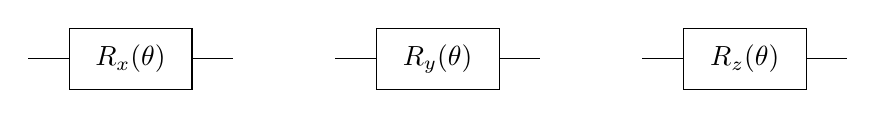
\begin{tikzpicture}[scale=1.3, >=stealth]
        % Gerbang R_x
        \draw (0,1) -- (2,1);
        \draw[fill=white] (0.4,0.7) rectangle (1.6,1.3) node[midway] {$R_x(\theta)$};
        
        % Gerbang R_y
        \draw (3,1) -- (5,1);
        \draw[fill=white] (3.4,0.7) rectangle (4.6,1.3) node[midway] {$R_y(\theta)$};
        
        % Gerbang R_z
        \draw (6,1) -- (8,1);
        \draw[fill=white] (6.4,0.7) rectangle (7.6,1.3) node[midway] {$R_z(\theta)$};
    \end{tikzpicture}
    \caption{Simbolisme gerbang rotasi pada sirkuit kuantum yang merepresentasikan rotasi parameter tunggal pada sumbu-X, sumbu-Y, dan sumbu-Z di bola Bloch.}
    \label{fig:gerbang_rotasi}
\end{figure}
\subsection{Manipulasi Informasi pada Gerbang 2 \textit{Qubit}}
Keterbelitan kuantum atau \textit{entanglement} merupakan fenomena non-lokal di mana keadaan satu \textit{qubit} tidak dapat didefinisikan secara independen dari keadaan \textit{qubit} lainnya dalam sistem multikomponen. Sebelum memahami keterbelitan pada sistem yang kompleks, perlu dipahami konsep Keadaan Bell (\textit{Bell States}) yang merupakan representasi dari keterbelitan maksimal antara dua \textit{qubit} terisolasi. Terdapat empat jenis Keadaan Bell yang membentuk basis ortonormal bagi ruang Hilbert dua-\textit{qubit} untuk merangkum seluruh probabilitas korelasi sistem fisis:
\begin{equation}
\label{eq:bell_states}
    |\Phi^{\pm}\rangle = \frac{|00\rangle \pm |11\rangle}{\sqrt{2}}, \quad |\Psi^{\pm}\rangle = \frac{|01\rangle \pm |10\rangle}{\sqrt{2}}.
\end{equation}
Keadaan Bell menunjukkan korelasi non-klasik yang sangat kuat, di mana tindakan pengukuran pada satu \textit{qubit} akan secara instan menentukan status keadaan \textit{qubit} lainnya meskipun keduanya terpisah secara fisik.

Pembangkitan keadaan Bell tersebut secara teknis dapat direkonstruksi dari basis komputasi dua \textit{qubit} melalui kombinasi linear gerbang Hadamard satu \textit{qubit} dengan gerbang dua \textit{qubit} \textit{Controlled-NOT} (CNOT)~\cite{mitarai_quantum_2018,innan_quantum_2025}. Secara matematis, langkah awal dilakukan dengan menerapkan transformasi gerbang Hadamard pada \textit{qubit} pertama yang diikuti dengan operasi identitas pada \textit{qubit} kedua:
\begin{equation}
(H\otimes I)|00\rangle = \frac{|00\rangle + |10\rangle}{\sqrt{2}}.
\end{equation}
Setelah itu, penerapan \textit{operator} CNOT pada keadaan superposisi tersebut memicu efek keterbelitan maksimal yang menghasilkan keadaan Bell pertama secara presisi:
\begin{equation}
\text{CNOT}\left(\frac{|00\rangle + |10\rangle}{\sqrt{2}}\right) = \frac{|00\rangle + |11\rangle}{\sqrt{2}} = |\Phi^+\rangle.
\end{equation}

Bentuk umum pemetaan dari seluruh basis komputasi dua \textit{qubit} menuju himpunan basis keadaan Bell tersebut dapat dituliskan secara komprehensif melalui relasi persamaan \textit{uniter} berikut:
\begin{equation}
\label{eq:bell_transformations}
\begin{split}
|\Phi^+\rangle &= \text{CNOT}(H\otimes I)|00\rangle, \quad |\Psi^+\rangle = \text{CNOT}(H\otimes I)|01\rangle, \\
|\Phi^-\rangle &= \text{CNOT}(H\otimes I)|10\rangle, \quad |\Psi^-\rangle = \text{CNOT}(H\otimes I)|11\rangle.
\end{split}
\end{equation}
Persamaan pemetaan uniter tersebut membuktikan bahwa \textit{operator} transformasi gabungan $U_{\text{Bell}} = \text{CNOT}(H\otimes I)$ secara fisis memetakan basis komputasi menuju basis Bell terbelit secara sempurna. Melalui formulasi perkalian luar (\textit{outer product}), representasi \textit{operator} transformasi basis kuantum tersebut dapat dituliskan secara rinci sebagai jumlahan proyeksi keadaan sebagai berikut:
\begin{equation}
\label{eq:u_bell_outer}
U_{\text{Bell}} = |\Phi^+\rangle\langle 00| + |\Psi^+\rangle\langle 01| + |\Phi^-\rangle\langle 10| + |\Psi^-\rangle\langle 11|.
\end{equation}

Untuk mendapatkan \textit{operator} CNOT dari representasi basis Bell, persamaan gabungan tersebut dikalikan dengan \textit{operator} invers dari transformasi Hadamard dari arah kanan. Karena \textit{operator} Hadamard bersifat \textit{self-inverse} yang berarti memiliki nilai invers sama dengan \textit{matriks} asalnya, maka \textit{operator} CNOT dapat ditransformasikan secara aljabar:
\begin{equation}
\label{eq:cnot_from_bell}
\text{CNOT} = U_{\text{Bell}}(H\otimes I) = \Big( |\Phi^+\rangle\langle 00| + |\Psi^+\rangle\langle 01| + |\Phi^-\rangle\langle 10| + |\Psi^-\rangle\langle 11| \Big) (H\otimes I).
\end{equation}
Persamaan di atas menunjukkan bahwa \textit{operator} CNOT dapat dibangun sepenuhnya dari deskripsi keadaan Bell dan transformasi Hadamard pada sistem kuantum. Dengan memasukkan definisi dari masing-masing keadaan Bell pada persamaan (\ref{eq:bell_states}) ke dalam perkalian luar tersebut, diperoleh representasi \textit{matriks} \textit{operator} \textit{uniter} yang mewakili gerbang tersebut.

Sebagai alternatif konstruksi langsung tanpa melibatkan gerbang Hadamard, \textit{operator} CNOT juga dapat didefinisikan secara langsung melalui aksi pemetaan basis komputasi~\cite{peruzzo_variational_2014}. Aksi pemetaan tersebut membalikkan status keadaan \textit{qubit} target apabila status keadaan \textit{qubit} kontrol bernilai satu, yang secara aljabar dituliskan sebagai:
\begin{equation}
\label{eq:cnot_actions}
\text{CNOT}|00\rangle = |00\rangle, \quad \text{CNOT}|01\rangle = |01\rangle, \quad \text{CNOT}|10\rangle = |11\rangle, \quad \text{CNOT}|11\rangle = |10\rangle.
\end{equation}
Dengan menggunakan aksi pemetaan basis komputasi tersebut, formulasi perkalian luar dari \textit{operator} CNOT dapat didefinisikan secara langsung melalui relasi jumlahan proyeksi keadaan:
\begin{equation}
\label{eq:cnot_outer_direct}
\text{CNOT} = |00\rangle\langle 00| + |01\rangle\langle 01| + |11\rangle\langle 10| + |10\rangle\langle 11|.
\end{equation}
Melalui evaluasi bentuk perkalian luar tersebut pada basis komputasi dua \textit{qubit}, \textit{matriks} \textit{uniter} dari gerbang CNOT dapat diturunkan secara eksplisit sesuai dengan arah kontrolnya:
\begin{equation}
\label{eq:cnot_matrices}
\text{CNOT}_{01} = \begin{pmatrix} 1 & 0 & 0 & 0 \\ 0 & 1 & 0 & 0 \\ 0 & 0 & 0 & 1 \\ 0 & 0 & 1 & 0 \end{pmatrix}, \quad \text{CNOT}_{10} = \begin{pmatrix} 1 & 0 & 0 & 0 \\ 0 & 0 & 0 & 1 \\ 0 & 0 & 1 & 0 \\ 0 & 1 & 0 & 0 \end{pmatrix}.
\end{equation}

Dalam konteks optimasi portofolio finansial, fenomena \textit{entanglement} dimanfaatkan secara cerdas untuk merepresentasikan hubungan ketergantungan dan \textit{matriks} korelasi silang antar berbagai variabel aset ekonomi secara efisien. Representasi visual dari mekanisme operasional gerbang CNOT diilustrasikan pada Gambar \ref{fig:gerbang_cnot}, yang secara rinci menunjukkan interaksi antara \textit{qubit} kontrol dengan titik hitam ($\bullet$) dan \textit{qubit} target dengan simbol plus dilingkari ($\oplus$).
\begin{figure}[htbp]
    \centering
    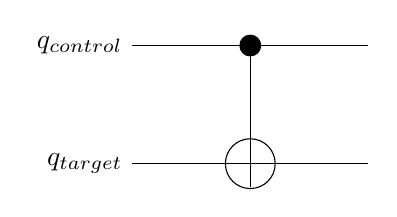
\begin{tikzpicture}[scale=1.5, >=stealth]
        \draw (0,1.5) -- (2,1.5) node[pos=0, left] {$q_{control}$};
        \draw (0,0.5) -- (2,0.5) node[pos=0, left] {$q_{target}$};
        \filldraw (1,1.5) circle (2.5pt);
        \draw (1,1.5) -- (1,0.5);
        \draw (1,0.5) circle (6pt);
        \draw (1,0.3) -- (1,0.7);
        \draw (0.8,0.5) -- (1.2,0.5);
    \end{tikzpicture}
    \caption{Representasi simbolik gerbang keterbelitan (\textit{Controlled-NOT}) yang mengilustrasikan interaksi non-lokal antar \textit{qubit} dalam sistem sirkuit.}
    \label{fig:gerbang_cnot}
\end{figure}

\subsection{Sirkuit Kuantum Berparameter}
\textit{Quantum Machine Learning} (QML) merupakan bidang multidisipliner yang menggabungkan prinsip komputasi kuantum dengan metode pemelajaran mesin. Salah satu pendekatan yang berkembang dalam QML adalah \textit{Quantum Deep Learning} (QDL), yaitu pemanfaatan model kuantum dengan parameter khusus untuk mempelajari pemodelan data kompleks. Implementasi model QDL umumnya diwujudkan melalui \textit{Parameterized Quantum Circuit} (PQC), yaitu sirkuit kuantum yang terdiri atas gerbang-gerbang kuantum yang memiliki parameter yang nilainya dapat dioptimasi. PQC menjadi komponen utama dalam keluarga \textit{Variational Quantum Algorithms} (VQA), yaitu algoritma hibrida yang menggabungkan pemrosesan kuantum dan optimasi klasik. Keluarga VQA terdiri dari \textit{Variational Quantum Eigensolver} (VQE), \textit{Quantum Approximate Optimization Algorithm} (QAOA), dan Variational Quantum Classifier (VQC) yang mana semuanya memanfaatkan PQC sebagai representasi solusi yang dievaluasi untuk kemudian nilainya diperbarui oleh algoritma optimasi klasik secara iteratif~\cite{reifenstein_coherent_2021,anshu_sample-efficient_2020,chen_enhanced_2025}.

Sirkuit Kuantum Berparameter (\textit{Parameterized Quantum Circuit} atau PQC) adalah rangkaian gerbang kuantum yang memiliki parameter kontinu, umumnya berupa sudut rotasi. Dalam algoritma variasional, rangkaian PQC berperan sebagai ansatz yang mengeksplorasi parameter pada ruang solusi untuk fungsi gelombang dari suatu permasalahan. Pada umumnya, alur kerja PQC ditunjukkan pada Gambar \ref{fig:pqc_workflow}. Secara singkat, proses diawali dengan penyandian data klasik $x \in \mathbb{R}^n$ ke dalam keadaan kuantum $|\psi_0\rangle$ melalui fungsi prapemrosesan $f(x)$ dan operasi penyandian $R(f(x))$. Keadaan kuantum yang telah terbentuk kemudian diproses oleh sirkuit variasional $U(\boldsymbol{\theta})$, yang bertugas mentransformasikan keadaan kuantum melalui serangkaian operasi kuantum berparameter. Parameter $\boldsymbol{\theta}$ pada sirkuit ini akan diperbarui secara iteratif selama proses optimasi untuk menghasilkan suatu keadaan kuantum $|\psi(\boldsymbol{\theta})\rangle$ yang merepresentasikan solusi optimum. Selanjutnya, keadaan akhir diproyeksikan melalui pengukuran $\{M\}$ untuk memperoleh nilai ekspektasi atau probabilitas observabel yang relevan. Hasil pengukuran tersebut kemudian dievaluasi menggunakan fungsi biaya $L(\boldsymbol{\theta})$, yang digunakan oleh algoritma optimasi klasik untuk menentukan pembaruan parameter hingga diperoleh parameter optimal $\boldsymbol{\theta}^∗$ dan keluaran model $y \in \mathbb{R}^n$.
\begin{figure}[htbp]
    \centering
    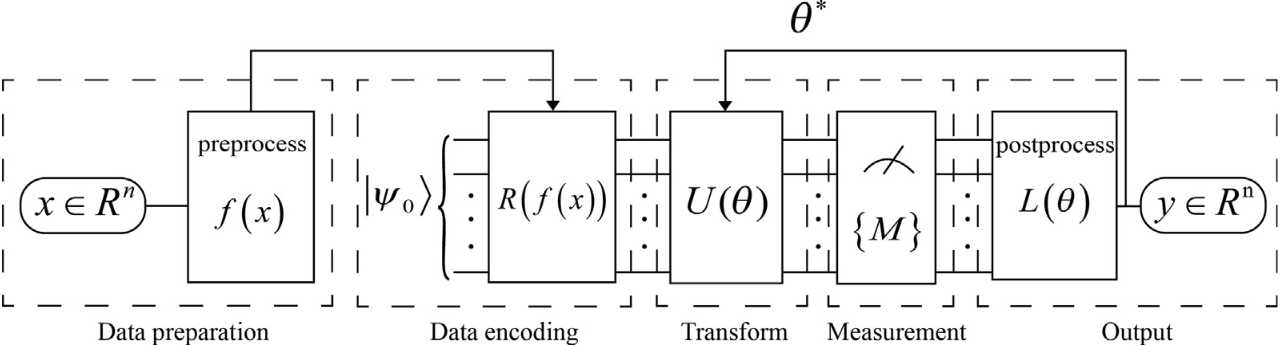
\includegraphics[width=0.7\textwidth]{Images/PQC_VQDNN.png}
    \caption[Representasi alur kerja sirkuit kuantum berparameter (PQC) yang mengilustrasikan tahap penyandian data, sirkuit variasional, pengukuran, dan pembaruan parameter oleh algoritma optimasi klasik \cite{regadio_exoplanet_2025}
    \label{fig:pqc_workflow}
\end{figure}

Setelah data dikodekan ke dalam keadaan kuantum $|\psi(\boldsymbol{\theta})\rangle$, sirkuit variasional $U(\boldsymbol{\theta})$ diterapkan untuk menghasilkan keadaan kuantum yang bergantung pada parameter-parameter optimasi. Berdasarkan sifat evolusi uniter dalam mekanika kuantum, keadaan keluaran sirkuit dapat dituliskan sebagai
\begin{equation}
\label{eq:vqa_state}
|\psi(\boldsymbol{\theta})\rangle = U(\boldsymbol{\theta})|\psi_0\rangle.
\end{equation}
di mana operator variasional $U(\boldsymbol{\theta})$ dibangun dari kombinasi gerbang rotasi satu-qubit dan gerbang keterbelitan dua-qubit. Secara umum, operator tersebut dapat dinyatakan
\begin{equation}
    U(\boldsymbol{\theta}) = \prod_{l=1}^L U_{(ent)}^{(l)} U_{(rot)}^{(l)} (\boldsymbol{\theta}^{(l)})
\end{equation}
dengan $U_{(rot)}^{(l)}$ merepresentasikan lapisan gerbang rotasi berparameter, seperti $Rx(\theta)$, $Ry(\theta)$, dan $Rz (\theta)$, sedangkan $U_{(ent)}^{(l)}$ menyatakan lapisan gerbang keterbelitan, misalnya gerbang CNOT. Struktur berlapis ini memungkinkan sirkuit menghasilkan keadaan kuantum yang semakin kompleks seiring bertambahnya jumlah parameter dan lapisan yang digunakan. Variasi nilai parameter $\boldsymbol{\theta}$ akan menghasilkan fungsi gelombang yang berbeda sehingga memungkinkan eksplorasi berbagai kandidat solusi di dalam ruang pencarian.

Kualitas suatu kandidat solusi kemudian dievaluasi melalui pengukuran nilai ekspektasi suatu operator observabel $\hat{O}$, yang umumnya merepresentasikan fungsi biaya atau besaran fisik yang ingin dioptimalkan. Nilai fungsi biaya tersebut dirumuskan sebagai
\begin{equation}
\label{eq:vqa_cost}
C(\boldsymbol{\theta}) = \langle \psi(\boldsymbol{\theta})| \hat{O} |\psi(\boldsymbol{\theta})\rangle.
\end{equation}
Nilai hasil pengukuran tersebut kemudian dikirimkan kepada \textit{optimizer} klasik untuk memperbarui parameter sirkuit, kemudian proses evaluasi dan pembaruan diulang hingga kriteria konvergensi terpenuhi. Proses ini dikenal sebagai \textit{hybrid quantum-classical optimization} atau optimasi hibrida kuantum-klasik.


\subsection{Pengukuran Kuantum}
Pengukuran merupakan tahap yang menghubungkan informasi kuantum dengan hasil observasi klasik yang dapat diakses oleh pengguna. Dalam mekanika kuantum, setiap besaran fisik direpresentasikan oleh suatu operator observabel Hermitian $\hat{O}$ yang memiliki himpunan nilai eigen $o_n$ dan vektor eigen ortonormal $|e_n\rangle$. Hubungan antara observabel dan basis eigennya dinyatakan melalui persamaan
\begin{equation}
\hat{O}|e_n\rangle = o_n |e_n\rangle.
\end{equation}
Jika suatu sistem berada pada keadaan $|\psi\rangle$, maka hasil pengukuran yang mungkin diperoleh hanyalah nilai-nilai eigen dari operator observabel tersebut. Untuk sebuah qubit yang berada pada keadaan superposisi
\begin{equation}
|\psi\rangle = a|0\rangle + b|1\rangle,
\end{equation}
probabilitas diperolehnya suatu hasil pengukuran ditentukan oleh kaidah Born (\textit{Born rule}). tersebut menyatakan bahwa probabilitas untuk memperoleh nilai eigen $o_n$ diberikan oleh proyeksi keadaan terhadap basis eigen observabel,
\begin{equation}
P(o_n) = |\langle e_n|\psi\rangle|^2.
\end{equation}
Sehingga, pada basis komputasi, probabilitas diperolehnya keadaan $|0\rangle$ dan $|1\rangle$ menjadi
\begin{equation} P(0)=|a|^2, \qquad P(1)=|b|^2.
\end{equation}
Hal tersebut menginterpretasi probabilistik ini menunjukkan bahwa hasil pengukuran tidak dapat diprediksi secara deterministik untuk satu percobaan tunggal, melainkan hanya dapat diprediksi melalui distribusi probabilitas hasil pengukuran.

Secara matematis, proses pengukuran direpresentasikan menggunakan operator proyeksi
\begin{equation} \hat{P}_n = |e_n\rangle\langle e_n|.
\end{equation}
Jika hasil pengukuran yang diperoleh adalah nilai eigen $o_n$, maka keadaan sistem setelah pengukuran diberikan oleh
\begin{equation}
|\psi'\rangle = \frac{\hat{P}_n|\psi\rangle} {\sqrt{\langle\psi|\hat{P}_n|\psi\rangle}}.
\end{equation}
Persamaan tersebut menunjukkan bahwa pengukuran menyebabkan sistem kehilangan superposisinya dan bertransisi menuju salah satu keadaan eigen observabel. Fenomena tersebut dikenal sebagai keruntuhan keadaan kuantum (\textit{state collapse}), yaitu perubahan non-unitari dari superposisi beberapa kemungkinan hasil menuju satu keadaan yang terdefinisi secara pasti. Mekanisme fisik yang menyebabkan hilangnya interferensi kuantum dapat dipahami melalui representasi matriks densitas. Untuk keadaan murni
\begin{equation}
|\psi\rangle = a|0\rangle+b|1\rangle,
\end{equation}
matriks densitas sistem didefinisikan sebagai
\begin{equation}
\rho = |\psi\rangle\langle\psi|.
\end{equation}
Dengan melakukan perkalian luar (\textit{outer product}), diperoleh
\begin{equation}
\begin{split}
\rho &= (a|0\rangle+b|1\rangle) (a^*\langle0|+b^*\langle1|)\\
&= |a|^2|0\rangle\langle0|+ ab^*|0\rangle\langle1| + a^*b|1\rangle\langle0| + |b|^2|1\rangle\langle1|.
\end{split}
\end{equation}
Dalam basis komputasi, bentuk tersebut dapat dituliskan sebagai
\begin{equation}
\rho=
\begin{bmatrix}
|a|^2 & ab^*\\
a^*b & |b|^2
\end{bmatrix}
\end{equation}
di mana elemen diagonal menyatakan probabilitas populasi masing-masing keadaan basis, sedangkan elemen \textit{off-diagonal} merepresentasikan koherensi kuantum yang bertanggung jawab terhadap fenomena interferensi.

Pada dasarnya, sistem kuantum tidak pernah sepenuhnya terisolasi dari lingkungan. Ketika sistem berinteraksi dengan lingkungan, keadaan gabungan sistem-lingkungan dapat dituliskan sebagai
\begin{equation}
|\Psi\rangle
=
a|0\rangle|e_0\rangle
+
b|1\rangle|e_1\rangle.
\end{equation}
Matriks densitas sistem kemudian diperoleh melalui operasi \textit{partial trace} terhadap derajat kebebasan lingkungan,
\begin{equation}
\rho_S
=
\mathrm{Tr}_E
\left(
|\Psi\rangle\langle\Psi|
\right),
\end{equation}
yang menghasilkan
\begin{equation}
\rho_S=
\begin{bmatrix}
|a|^2 &
ab^*\langle e_1|e_0\rangle\\
a^*b\langle e_0|e_1\rangle &
|b|^2
\end{bmatrix}.
\end{equation}
Keberadaan faktor $\langle e_1|e_0\rangle$ menunjukkan bahwa koherensi sistem bergantung pada tingkat tumpang tindih keadaan lingkungan yang berkorelasi dengan masing-masing keadaan basis qubit. Namun seiring bertambahnya interaksi dengan lingkungan, keadaan lingkungan menjadi semakin ortogonal sehingga
\begin{equation}
\langle e_1|e_0\rangle
\rightarrow 0.
\end{equation}
Sehingga elemen-elemen \textit{off-diagonal} menghilang dan matriks densitas sistem mereduksi menjadi
\begin{equation}
\rho_S
\rightarrow
\begin{bmatrix}
|a|^2 & 0\\
0 & |b|^2
\end{bmatrix}.
\end{equation}
Proses hilangnya koherensi kuantum ini dikenal sebagai dekoherensi (\textit{decoherence}) yaitu mengubah keadaan kuantum menjadi campuran statistik yang tidak lagi menunjukkan interferensi.

Secara konsep, hubungan antara dekoherensi dan keruntuhan keadaan kuantum tersebut dapat direpresentasikan pada Gambar \ref{fig:collapse_measurement}. Gambar tersebut memperlihatkan bagaimana elemen \textit{off-diagonaal} yang merepresentasikan koherensi kuantum secara bertahap menghilang akibat interaksi dengan lingkungan, menghasilkan matriks densitas diagonal yang bersifat statistik. Setelah itu, proses pengukuran memproyeksikan sistem ke salah satu keadaan basis yang terdefinisi secara pasti sesuai probabilitas yang diberikan oleh kaidah Born.

\begin{figure}[htbp]
    \centering
    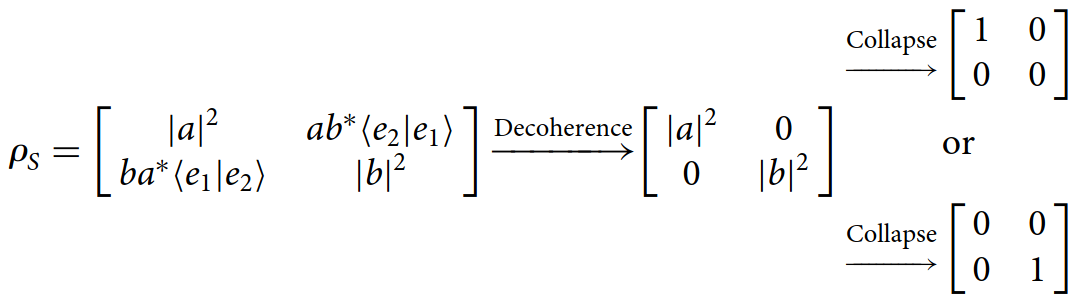
\includegraphics[width=\textwidth]{Images/Collapse_Measurement.png}
    \caption{Representasi konseptual hubungan antara dekoherensi dan keruntuhan keadaan kuantum. Interaksi sistem dengan lingkungan menyebabkan hilangnya elemen koherensi (\textit{off-diagonaal}) pada matriks densitas, sedangkan proses pengukuran memproyeksikan sistem ke salah satu keadaan eigen yang terdefinisi.}
    \label{fig:collapse_measurement}
\end{figure}